\documentclass[11pt]{article}
\usepackage{amsmath,amssymb,amsthm}
\usepackage[letterpaper,margin=1in]{geometry}
\usepackage{microtype}
\usepackage{graphicx}
\usepackage{tikz}
\usepackage[hidelinks]{hyperref}
\newtheorem{theorem}{Theorem}
\newtheorem{lemma}[theorem]{Lemma}
\newtheorem{corollary}[theorem]{Corollary}
\newtheorem{proposition}[theorem]{Proposition}
\newcommand{\R}{\mathbb R}
\newcommand{\cut}{\chi}
\title{Planar Steiner diversities need logarithmic\texorpdfstring{\\ $\ell_1$}{ L1} distortion}
\author{Jeff Kline}
\date{Pre-release draft --- 2026-10-25}
\hypersetup{pdftitle={Planar Steiner diversities need logarithmic L1 distortion},pdfauthor={Jeff Kline}}
\begin{document}
\maketitle
\begin{center}\small Pre-release draft. Not admitted, not peer reviewed.\end{center}
\begin{abstract}
The Steiner diversity of a graph assigns to each vertex set the minimum cost
of a connected subgraph containing it. On unit diamond graphs, this diversity
requires logarithmic distortion in $\ell_1$, although the graphs are planar
and have treewidth two. After $d\ge1$ edge-replacement rounds the graph has
$N_d=(2\cdot4^d+4)/3$ vertices, and we prove the explicit lower bound
$c_1(D_d)\ge(6d+7+2/4^d)/9$. A cut inequality on the nested generation sets,
together with their exact Steiner costs, gives a rational dual certificate
with only $d$ demand sets. Combined with Bryant and Tupper's upper bound for
metric Steiner diversities, the result has order $\log N_d$. The same
certificate supplies unit-capacity set demands that satisfy every cut
condition but require at least this much routing congestion. The exact value
of $c_1(D_d)$ is not determined for $d\ge3$. Three bounded literature scans
found no matching result; novelty remains unresolved.
\end{abstract}

\section{Introduction}
The Steiner diversity of a graph assigns to each vertex set the minimum cost
of a connected subgraph containing it. On unit diamond graphs, this diversity
requires logarithmic distortion in $\ell_1$, although the graphs are planar
and have treewidth two. The obstruction concerns one embedding that must
preserve the connection costs of all terminal sets simultaneously.

A diversity extends a metric from pairs to finite sets. For a finite set $V$,
it is a function $\delta:2^V\to[0,\infty)$ that vanishes exactly on sets of
size at most one and satisfies
\[
\delta(A\cup B)\le\delta(A\cup C)+\delta(C\cup B)
\qquad(C\ne\varnothing).
\]
Bryant and Tupper introduced this framework~\cite{BT12} and developed its
connection to hypergraph cuts and flows~\cite{BT14}. For a finite connected
graph $G=(V,E)$ with positive edge lengths $\ell$, its \emph{graph Steiner
diversity} is
\[
\delta_{G,\ell}(A)=\min\left\{\sum_{e\in E(H)}\ell(e):
 H\subseteq G\text{ is connected and }A\subseteq V(H)\right\},
\]
with value zero for $|A|\le1$. Every vertex of $G$ is available as a Steiner
point. Edges are ordinary pairs throughout this paper.

For $f:V\to\R^m$, the coordinate-range $\ell_1$ diversity is
\[
h_f(A)=\sum_{i=1}^m\left(\max_{v\in A}f_i(v)-\min_{v\in A}f_i(v)\right),
\]
again zero on the empty set. Write $c_1(\delta)$ for the infimum of $D\ge1$
over all finite dimensions and maps satisfying
$\delta(A)\le h_f(A)\le D\delta(A)$ for every $A\subseteq V$. Rescaling the
map permits this noncontracting normalization. For unit graph lengths we
write $c_1(G)$.

Recent metric results in OpenAI's Erd\H{o}s problem \#089 materials concern
constant-distortion embeddings for planar graphs and graphs of fixed
treewidth~\cite{OAIplanar,OAItw}. These are statements about pairs. For the
series-parallel class containing diamonds, the bound of two is attributed
to Chakrabarti, Jaffe, Lee and Vincent~\cite{CJLV}, as reported in
\cite[Section 1.2]{OAIplanar}. We use that attribution only as context;
we do not claim that diamond metrics embed isometrically. The question here
is whether a constant can also preserve every Steiner set cost. The answer
is no, already at treewidth two.

\paragraph{Results and scope.}
The principal result is the explicit all-depth bound in Theorem~\ref{thm:main}.
Its proof uses a simultaneous cut inequality on $d$ nested sets, rather than
pairwise separation. Corollaries~\ref{cor:order} and~\ref{cor:flow} give the
asymptotic order and a normalized set-demand flow--cut consequence. Secondary
results identify the exact optimum of the restricted certificate method and
its dependence on edge lengths. None of these statements determines the
full optimal distortion at depth three or beyond. The computational table
checks finite controls; it is not a premise of the proof. Prior work is
credited in Section~\ref{sec:earlier}. The three recorded searches were
bounded and source-negative, so novelty remains unresolved.

\section{The diamond lower bound}
Let $D_0$ be one edge. To obtain $D_d$ from $D_{d-1}$, replace every edge by
two internally disjoint paths of two edges each. Every final edge has unit
length. Retain all earlier vertices, and let $V_j$ be the vertex set present
after generation $j$, viewed as a subset of $V_d$.

\begin{theorem}\label{thm:main}
For every integer $d\ge1$, the graph $D_d$ has $4^d$ edges and
$N_d=(2\cdot4^d+4)/3$ vertices. It is planar and has treewidth exactly two.
Its graph Steiner diversity satisfies
\[
c_1(D_d)\ge L_d:=\frac{6d+7+2/4^d}{9}.
\]
Consequently, neither planar graphs nor graphs of treewidth two admit a
uniform constant bound on $\ell_1$ diversity distortion.
\end{theorem}

\subsection{Cut representation and duality}
For a cut $S\subseteq V$, let $\cut_S(A)$ be one if $A$ meets both $S$ and
$V\setminus S$, and zero otherwise. Every coordinate-range $\ell_1$ diversity
on a finite set is a finite nonnegative sum
\[
h(A)=\sum_S w_S\cut_S(A),\qquad w_S\ge0.
\]
Indeed, sort the distinct values of each coordinate and assign each
consecutive gap to its upper threshold cut. A set crosses exactly the
thresholds between its minimum and maximum. Conversely, the coordinate
$w_S\mathbf1_S$ realizes $w_S\cut_S$.

Suppose nonnegative measures $\alpha,\beta$ on subsets of $V$ satisfy
\begin{equation}\label{eq:dual}
\sum_A\alpha_A\cut_S(A)\le\sum_A\beta_A\cut_S(A)
\quad\text{for every }S,\qquad
\sum_A\beta_A\delta(A)=1.
\end{equation}
Then any $\delta\le h\le D\delta$ obeys
\[
\sum_A\alpha_A\delta(A)\le\sum_A\alpha_Ah(A)
\le\sum_A\beta_Ah(A)\le D.
\]
This is the dual-certificate principle used below. It applies in every
allowed finite dimension.

\subsection{Geometry and graph class}
Each replacement multiplies the number of edges by four and adds two
vertices per old edge. Thus
\[
E_d=4^d,\qquad N_d=2+2\sum_{i=0}^{d-1}4^i=\frac{2\cdot4^d+4}{3}.
\]
Each edge of $D_j$ has a descendant gadget isomorphic to $D_{d-j}$.
Distinct gadgets have disjoint edge sets and disjoint interiors, meeting
only at old endpoints. Within a gadget the terminal distance is $2^{d-j}$,
and there are $2^{d-j}$ edge-disjoint terminal paths. Both assertions follow
inductively: two smaller diamonds occur in series in each of two parallel
branches. Distances double; corresponding paths concatenate in each branch,
and the two branch collections are edge-disjoint.

Every edge of $D_j$, for $j\ge1$, lies in the four-cycle replacing its
parent edge. Hence $D_j$ is connected and bridgeless, and each nontrivial
cut crosses at least two edges.

Replacing each edge in a planar drawing inside a narrow neighborhood
preserves planarity. For a width-two tree decomposition, start with the
bag containing the original two endpoints. When $xy$ is replaced through
new vertices $a,b$, attach bags $\{x,y,a\}$ and $\{x,y,b\}$ to an existing
bag containing $x,y$. Old edge coverage ensures such a bag exists. The new
edges are covered, and the bags containing each vertex remain connected.
Retain old bags after their edges disappear. Every bag has size at most
three. Since $D_d$ contains a cycle for $d\ge1$, its treewidth is exactly two.

\begin{figure}[tb]
\centering
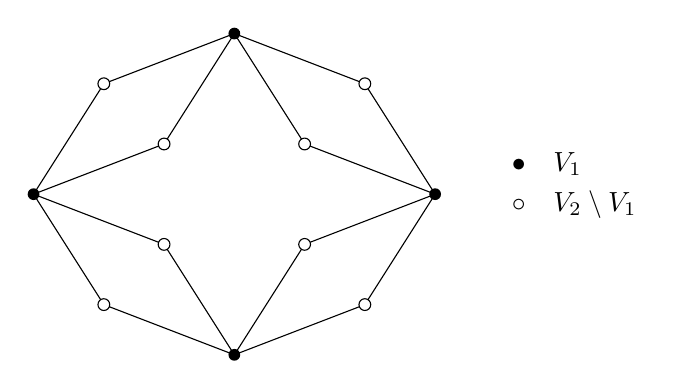
\begin{tikzpicture}[scale=0.85]
\coordinate (u) at (0,0); \coordinate (v) at (6,0);
\coordinate (a) at (3,2.4); \coordinate (b) at (3,-2.4);
\coordinate (p1) at (1.05,1.65); \coordinate (p2) at (1.95,0.75);
\coordinate (p3) at (4.05,0.75); \coordinate (p4) at (4.95,1.65);
\coordinate (p5) at (1.05,-1.65); \coordinate (p6) at (1.95,-0.75);
\coordinate (p7) at (4.05,-0.75); \coordinate (p8) at (4.95,-1.65);
\draw (u)--(p1)--(a)--(p2)--(u);
\draw (a)--(p3)--(v)--(p4)--(a);
\draw (u)--(p5)--(b)--(p6)--(u);
\draw (b)--(p7)--(v)--(p8)--(b);
\foreach \x in {u,v,a,b} \fill (\x) circle (2.5pt);
\foreach \x in {p1,p2,p3,p4,p5,p6,p7,p8}
  \draw[fill=white] (\x) circle (2.5pt);
\node[anchor=west] at (7,0.45) {$\bullet\quad V_1$};
\node[anchor=west] at (7,-0.15) {$\circ\quad V_2\setminus V_1$};
\end{tikzpicture}
\caption{The unit diamond $D_2$. All twelve vertices form $V_2$; the four
filled vertices form $V_1$. Their Steiner costs are respectively $11$ and $6$.
The drawing does not encode edge lengths.}
\label{fig:diamond}
\end{figure}

\subsection{A simultaneous inequality for every cut}
Set
\[
a_j=2^{d-j}\quad(1\le j<d),\qquad a_d=2.
\]
\begin{lemma}\label{lem:cut}
For every cut $S$ of $D_d$,
\begin{equation}\label{eq:cut}
\sum_{j=1}^d a_j\cut_S(V_j)\le |\partial_{D_d}S|.
\end{equation}
\end{lemma}
\begin{proof}
Trivial cuts have both sides zero. For a nontrivial cut, let $q$ be the first
generation in $\{1,\ldots,d\}$ with $\cut_S(V_q)=1$. It exists since $V_d$
is the whole vertex set. By nesting, the indicators vanish before $q$ and
are one thereafter. The restriction to $V_q$ is a nontrivial cut of $D_q$,
so it crosses at least two coarse edges. Their descendant gadgets are
edge-disjoint. In each, $S$ separates the endpoints and therefore crosses
all $2^{d-q}$ edge-disjoint terminal paths. Consequently
\[
|\partial_{D_d}S|\ge2^{d-q+1}=\sum_{j=q}^d a_j
=\sum_{j=1}^d a_j\cut_S(V_j).
\]
This includes $q=d$ and $d=1$.
\end{proof}

\subsection{Exact Steiner costs of the generation sets}
\begin{lemma}\label{lem:cost}
For $1\le j\le d$,
\begin{equation}\label{eq:cost}
\delta_{D_d}(V_j)=2^{d-j}(N_j-1).
\end{equation}
\end{lemma}
\begin{proof}
For the upper bound, choose a spanning tree of $D_j$ and a shortest terminal
path in each of its $N_j-1$ edge gadgets. Their union is connected, contains
$V_j$, and has $2^{d-j}(N_j-1)$ edges.

For the lower bound, let $H$ be any connected subgraph containing $V_j$.
Retain a coarse edge of $D_j$ whenever $H$ connects its endpoints within
its descendant gadget. The retained edges connect $V_j$: a simple $H$-path
between old vertices, divided at successive old vertices, consists of
passages through single gadgets between their endpoints. Different gadgets
meet only at old endpoints. Each passage gives a retained coarse edge.
At least $N_j-1$ gadgets are therefore retained. Each costs at least
$2^{d-j}$ edges, and their edge sets are disjoint. This proves the lower
bound even when $H$ uses arbitrary newer Steiner vertices.
\end{proof}

\subsection{The certificate and its objective}
Put $\alpha_{V_j}=a_j/4^d$ and put $\beta_{\{u,v\}}=1/4^d$ on every final
graph edge, with all other coefficients zero. Every edge pair has Steiner
cost one, so $\sum_A\beta_A\delta(A)=1$. Dividing~\eqref{eq:cut} by $4^d$
gives every cut constraint in~\eqref{eq:dual}. By~\eqref{eq:cost},
\begin{align*}
\sum_A\alpha_A\delta(A)
&=\frac1{4^d}\left[\sum_{j=1}^{d-1}
  \frac{4^{d-j}(2\cdot4^j+1)}3+\frac{2(2\cdot4^d+1)}3\right]\\
&=\frac{2(d-1)}3+\frac19\bigl(1-4^{-(d-1)}\bigr)
  +\frac43+\frac2{3\cdot4^d}\\
&=\frac{6d+7+2/4^d}{9}.
\end{align*}
The sum is empty when $d=1$. The dual-certificate principle proves
Theorem~\ref{thm:main}. Since $N_d$ is proportional to $4^d$,
$L_d=(2/3)\log_4N_d+O(1)$, which diverges.

\section{Consequences and limits}
\begin{corollary}\label{cor:order}
The unit diamond diversities have $c_1(D_d)=\Theta(\log N_d)$.
The lower bound is self-contained; the upper bound uses
\cite[Theorem 2]{BTopen}.
\end{corollary}
\begin{proof}
Bryant and Tupper prove an $O(\log n)$ upper bound for the Steiner diversity
of an $n$-point metric space. Graph Steiner costs equal the Steiner costs
in the shortest-path metric completion on the same vertex set. Replacing
metric-tree edges by graph shortest paths gives one inequality; viewing a
graph Steiner tree as a tree of metric edges gives the other. All vertices
remain available as Steiner points. The cited theorem and
Theorem~\ref{thm:main} now give the claimed order.
\end{proof}

\begin{corollary}[Set-demand flow--cut form]\label{cor:flow}
Give every edge of $D_d$ capacity one and give terminal set $V_j$ demand
$a_j$, with all other demands zero. These demands satisfy every cut
condition, but any fractional Steiner-tree routing of the full demands
requires congestion at least $L_d$. In the notation of
\cite[Section 5]{BT14},
\[
\mathrm{MinHypCut}=1,\qquad \mathrm{MaxHSP}\le L_d^{-1},\qquad
\frac{\mathrm{MinHypCut}}{\mathrm{MaxHSP}}\ge L_d.
\]
\end{corollary}
\begin{proof}
The cut condition is exactly~\eqref{eq:cut}. The cut ratio is boundary
capacity divided by $\sum_j a_j\cut_S(V_j)$, for nonzero denominator. Every
such ratio is at least one. A singleton vertex born in generation $d$
has degree two and crosses only the demand set $V_d$, whose demand is two;
its ratio is one.

For each $j$, distribute mass $a_j$ over trees containing $V_j$. The sum of
all edge loads is at least $\sum_j a_j\delta(V_j)=4^dL_d$. Congestion $\rho$
with unit capacities bounds that sum above by $\rho4^d$, hence
$\rho\ge L_d$. Bryant and Tupper's maximum concurrent packing variable
$f$ routes mass $fa_j$ under the original capacities. The same calculation
gives $f4^dL_d\le4^d$. This verifies the stated normalization directly.
Their Theorems 1--2 and 17--18 establish the general diversity/flow--cut
correspondence; the calculation here supplies these particular demands.
\end{proof}

\begin{proposition}[Secondary: length dependence]\label{prop:length}
Common positive rescaling of all edge lengths preserves $c_1$. If the
lengths on $D_d$ satisfy $0<m\le\ell(e)\le M$ and $R=M/m$, then
\[
c_1(D_d,\ell)\ge\max\{1,L_d/R\}.
\]
There are also strictly positive length assignments on every underlying
diamond for which $c_1=1$.
\end{proposition}
\begin{proof}
Common rescaling multiplies all Steiner costs and all embedding coordinates
by the same factor. For bounded lengths, minimizing over the same connected
subgraphs gives $m\delta_{\rm unit}\le\delta_\ell\le M\delta_{\rm unit}$.
If $\delta_\ell\le h\le D\delta_\ell$, then $h/m$ is noncontracting for
$\delta_{\rm unit}$ with distortion at most $DR$. Take infima and apply
Theorem~\ref{thm:main}.

For the last assertion, choose a spanning tree $T$ on $N$ vertices, give
its edges length one, and give every other edge length $N$. Every non-tree
edge can be replaced by its $T$-path of at most $N-1$ edges. Thus every
connected subgraph spanning $A$ can be replaced by one in $T$ of no greater
cost, and $\delta_{G,\ell}(A)=\delta_T(A)$ for every $A$. The tree diversity
is the sum of its edge-cut diversities, so it embeds exactly in $\ell_1$.
\end{proof}

\begin{proposition}[Secondary: optimum of the restricted method]\label{prop:method}
On the unit diamond, fix $\beta_{\{u,v\}}=1/4^d$ on every edge and require
$\alpha$ to be supported on $V_1,\ldots,V_d$. Among feasible nonnegative
$\alpha$ in~\eqref{eq:dual}, the maximum objective is $L_d$, uniquely attained
by the coefficients of Theorem~\ref{thm:main}.
\end{proposition}
\begin{proof}
Write $x_j=4^d\alpha_{V_j}$, $y_q=\sum_{j=q}^dx_j$, and
$b_q=2^{d-q+1}$. The all-cut feasible region is exactly
\[
x_j\ge0,\qquad y_q\le b_q\quad(1\le q\le d).
\]
Necessity follows from a singleton vertex born in generation $q$: its degree
is $b_q$, and it crosses exactly the generation sets indexed at least $q$.
For sufficiency, the proof of Lemma~\ref{lem:cut} bounds any cut first
splitting $V_q$ below by $b_q$ boundary edges.

Let $c_j=\delta(V_j)$. Lemma~\ref{lem:cost} gives $c_1>0$ and
$c_j-c_{j-1}=2^{d-j}(4^j-1)/3>0$ for $j\ge2$. Summation by parts yields
\[
4^{-d}\sum_{j=1}^dc_jx_j
=4^{-d}\left(c_1y_1+\sum_{j=2}^d(c_j-c_{j-1})y_j\right).
\]
Every coefficient is positive, so the maximum requires $y_q=b_q$ for all
$q$. These equalities are simultaneously feasible since $b_q$ decreases.
They give $x_j=b_j-b_{j+1}=2^{d-j}$ for $j<d$ and $x_d=2$, as claimed.
\end{proof}

This restricted optimality does not establish the full dual optimum or
$c_1(D_d)=L_d$ for $d\ge3$. Uniform lengths provide the witness family;
Theorem~\ref{thm:main} is not a lower bound for every positive-length diamond.
The result concerns graph Steiner diversities with arbitrary graph vertices
as Steiner points, and finite-dimensional coordinate-range $\ell_1$ targets.
It is not a claim about terminal-induced subgraphs, terminal-only Steiner
trees, or the distortion of pairs alone.

\section{Exact finite controls}
Table~\ref{tab:cases} records 28 saved rational primal/dual certificates.
The draft verifier constructs $D_1,D_2$, checks every cut, enumerates exact
Steiner costs, checks the objective identity for $d=1,\ldots,12$, and checks
all 28 certificates. No new linear programs are solved. On each saved graph,
the verifier computes the minimum spanning-tree cost on every induced vertex
set, then minimizes over supersets of each terminal set. This gives exact
Steiner costs because any connected subgraph contains a spanning tree.
It checks both bounds on every terminal set, all dual cut constraints,
normalization, and equality of primal and dual objectives using rational
arithmetic. These finite checks do not verify the all-depth theorem.

\begin{table}[tb]
\centering
\begin{tabular}{lr@{\qquad}lr}
\hline
Graph & Exact $c_1$ & Graph & Exact $c_1$\\
\hline
Path, 8 vertices & $1$ & $D_2$ & $17/8$\\
Star, 8 vertices & $1$ & Fan, 5 vertices & $8/5$\\
$K_3$ & $4/3$ & Fan, 8 vertices & $7/4$\\
$K_4$ & $3/2$ & Wheel, 5 vertices & $5/3$\\
$K_5$ & $8/5$ & Wheel, 8 vertices & $38/21$\\
$K_6$ & $5/3$ & Grid $2\times3$ & $5/3$\\
$K_8$ & $7/4$ & Grid $2\times4$ & $7/4$\\
$C_4$ & $3/2$ & Grid $2\times5$ & $9/5$\\
$C_5$ & $8/5$ & Grid $2\times6$ & $11/6$\\
$C_6$ & $5/3$ & Grid $3\times3$ & $11/6$\\
$C_7$ & $12/7$ & Grid $3\times4$ & $29/15$\\
$C_8$ & $7/4$ & Weighted 2-tree, seed 17 & $4/3$\\
$C_{10}$ & $9/5$ & Weighted 2-tree, seed 31 & $14/11$\\
$C_{12}$ & $11/6$ & Weighted 2-tree, seed 53 & $26/19$\\
\hline
\end{tabular}
\caption{Exact certificate values. Fans and wheels count all vertices,
including the hub. The path has edge lengths $1,2,3$ repeated, the star has
lengths $1,\ldots,7$, and each 2-tree has eight vertices and recorded integer
lengths in $1,\ldots,9$. All other edges have unit length.}
\label{tab:cases}
\end{table}

All 28 final saved solver records report optimal status, and the exact
certificate checks remove reliance on floating-point tolerances for these
values. Three initial full formulations had timed out; the saved successful
runs used an equivalent reduction to upper constraints on edges and retained
all lower constraints. The present verifier checks every upper constraint
as well, so it does not rely on that reduction. The equalities
$c_1(D_1)=3/2$ and $c_1(D_2)=17/8$ match $L_1,L_2$; they do not justify
extrapolating equality to larger depths.

\section{Earlier work and unresolved priority}\label{sec:earlier}
Bryant and Tupper supply the diversity framework~\cite{BT12}, the cut
representation and hypergraph flow--cut connection~\cite{BT14}, and the
$O(\log n)$ Steiner-diversity upper bound~\cite[Theorem 2]{BTopen}.
We cite the last result as an external dependency; its random-tree argument
has not been independently audited here. The arXiv record identifies a 2017
version, although the saved PDF prints an October 2021 date.

Jozefiak and Shepherd~\cite{JS} discuss a general-graph logarithmic lower
bound inherited from expander metrics. That argument does not establish the
planar, treewidth-two statement here. Gupta, Newman, Rabinovich and
Sinclair~\cite{GNRS} prove logarithmic lower bounds for embeddings of
series-parallel metrics into distributions of dominating trees. This is a
nearby metric result with a different target. Their publisher abstract was
checked; the full article was not inspected for this draft. The
series-parallel $\ell_1$ metric bound attributed to~\cite{CJLV} was read in
the OpenAI papers' discussion, not in the original conference paper.

The author's earlier paper~\cite{Kline} concerns hypergraph Steiner
diversities and an affine covering-versus-hitting construction. Its
hyperedges may contain more than two vertices. The present witness consists
entirely of graph edges and uses nested diamond generations.

Three saved bounded scans searched diversity terminology, flow--cut
terminology, and selected citing papers. They found no source containing the
same planar graph-Steiner lower bound or its generation-set certificate.
That negative outcome is not a priority certificate. Search coverage,
access failures, citations inspected only at abstract level, and unresolved
candidates are recorded in the repository's prior-work audit. Novelty
remains unresolved, including at the level of the mechanism.

\section*{AI assistance and verification status}
AI systems assisted with the research, adversarial examination, finite
certificate checks, source extraction, and preparation of this draft. A
fresh full proof audit and the owner's adjudication are preserved as
unchanged evidence. An initial examiner's alternative argument was adopted
before that audit. The records distinguish an unsuccessful attempt to break
a claim from a subsequent proof review. Neither constitutes peer review or
formal proof-assistant certification. The author is responsible for the
mathematical claims and their presentation. This document is a pre-release
draft, not an admission or publication decision.

\begin{thebibliography}{9}
\bibitem{BT12} D. Bryant and P. F. Tupper.
Hyperconvexity and tight-span theory for diversities.
\emph{Advances in Mathematics} 231(6):3172--3198, 2012.
\bibitem{BT14} D. Bryant and P. F. Tupper.
Diversities and the Geometry of Hypergraphs.
\emph{Discrete Mathematics \& Theoretical Computer Science} 16(2):1--20, 2014.
\href{https://dmtcs.episciences.org/articles/2080}{Journal article}.
\bibitem{BTopen} D. Bryant and P. Tupper.
Open Problem Statement: Minimal Distortion Embeddings of Diversities in $\ell_1$.
\href{https://arxiv.org/abs/1712.01960v1}{arXiv:1712.01960v1}, 2017.
\bibitem{JS} A. D. Jozefiak and F. B. Shepherd.
Diversity Embeddings and the Hypergraph Sparsest Cut.
\href{https://arxiv.org/abs/2303.04199v1}{arXiv:2303.04199v1}, 2023.
\bibitem{OAIplanar} OpenAI.
Planar Graph Metrics Embed into L1 with Constant Distortion.
Preprint, September 23, 2026.
\href{https://github.com/openai/math/blob/main/lean/docs/089.md}{Official problem \#089 index}.
\bibitem{OAItw} OpenAI.
L1 Embeddings of Graphs of Bounded Treewidth.
Preprint, September 23, 2026.
\href{https://github.com/openai/math/blob/main/lean/docs/089.md}{Official problem \#089 index}.
\bibitem{CJLV} A. Chakrabarti, A. Jaffe, J. R. Lee and J. Vincent.
Embeddings of Topological Graphs: Lossy Invariants, Linearization, and 2-Sums.
In \emph{49th Annual IEEE Symposium on Foundations of Computer Science},
pages 761--770, 2008. Metadata and metric bound checked in \cite{OAIplanar,OAItw};
original paper not inspected.
\bibitem{GNRS} A. Gupta, I. Newman, Y. Rabinovich and A. Sinclair.
Cuts, Trees and $\ell_1$-Embeddings of Graphs.
\emph{Combinatorica} 24(2):233--269, 2004.
\bibitem{Kline} J. Kline.
Covering versus hitting in diversity embeddings: an affine obstruction and
matching bounds. Version 0.1.0, September 13, 2026.
\href{https://github.com/jeff-kline/covering-hitting-diversities}{Repository}.
\end{thebibliography}
\end{document}
